\chapter{燃烧：燃料、生成物与温室气体}\label{ch:g8:combustion-and-fuels}

一家人住在一套公寓里，其燃气锅炉的烟道堵塞了。火焰
因缺氧而燃烧得很差，一种看不见、没有气味的气体慢慢
充满房间。凌晨两点，墙上的一个小盒子开始
尖叫，那是一氧化碳报警器。所幸大家及时逃了出来。同样的
燃料充分燃烧时只生成二氧化碳和水——而这种
二氧化碳还有自己的故事，写在整个
地球的大气之中。

\begin{recall}
燃烧需要燃料、氧气和热量，并生成新的
物质（见\cref{ch:g4:what-a-fire-needs}）。空气中约五分之一为
氧气（见\cref{ch:g4:air-a-mixture-of-gases}）。方程式配平
是指等号两边每种原子出现的次数相同
（见\cref{ch:g8:balanced-equations}）。
\end{recall}

\section{碳与甲烷的燃烧}

\begin{example}[两种燃烧]\label{ex:g8:combustion-and-fuels:two}
碳（木炭、煤）燃烧生成二氧化碳：
\[
  \ce{C(s) + O2(g) -> CO2(g)}.
\]
甲烷是天然气的主要成分，燃烧生成二氧化碳和
水：
\[
  \ce{CH4(g) + 2O2(g) -> CO2(g) + 2H2O(l)}.
\]
两种情况下，生成的气体都会使石灰水变浑浊；
燃烧甲烷时，冷玻璃上还会起雾。
\end{example}

\begin{method}[写出由碳、氢组成的燃料的燃烧方程式]\label{met:g8:combustion-and-fuels:write}
对于分子中只含碳和氢的燃料：
\begin{enumerate}
  \item 生成物为二氧化碳和水；
  \item 先用 \ce{CO2} 配平碳，再用 \ce{H2O} 配平氢；
       \item 数出右边的氧原子数，并用
        \ce{O2} 配平；若出现分数系数，则将全部系数乘以 2。
\end{enumerate}
对于丁烷：\ce{2C4H10 + 13O2 -> 8CO2 + 10H2O}。
\end{method}

\section{完全燃烧与不完全燃烧}

\begin{definition}[完全燃烧与不完全燃烧]\label{def:g8:combustion-and-fuels:complete}
氧气充足时发生的燃烧称为\emph{完全燃烧}\index{完全燃烧}，
燃料中的碳全部变为二氧化碳。
而\emph{不完全燃烧}\index{不完全燃烧}发生在
氧气不足时，部分碳变为一氧化碳，
\ce{CO}，或变为炭黑；炭黑即碳 \ce{C}。
\end{definition}

\begin{example}[氧气不足时的甲烷]\label{ex:g8:combustion-and-fuels:incomplete}
空气不足时，甲烷可燃烧生成一氧化碳或炭黑：
\[
  \ce{2CH4 + 3O2 -> 2CO + 4H2O}, \qquad \ce{CH4 + O2 -> C + 2H2O}.
\]
\end{example}

\begin{proposition}[读懂火焰]\label{prop:g8:combustion-and-fuels:flame}
打开进气孔的本生灯，燃烧前先将空气与燃气
混合后再燃烧：火焰呈蓝色且几乎不可见，燃烧完全。
进气孔关闭时，燃气得不到足够的氧气：火焰
呈黄色且有烟，并使置于其中的冷物体覆上炭黑——
此时燃烧不完全。
\end{proposition}

\begin{omfigure}
\begin{tikzpicture}[font=\small, scale=1.3]
  \pic[transform shape] at (0,0) {bunsen=open};
  \node[anchor=north, align=center] at (0,-0.1) {进气孔打开：\\ 蓝色火焰，完全燃烧};
  \pic[transform shape] at (4,0) {bunsen=closed};
  \node[anchor=north, align=center] at (4,-0.1) {进气孔关闭：\\ 黄色火焰，不完全燃烧};
  \draw[<-, omProp, thick] (0.08,0.6) -- (1.4,0.9) node[right, text=black] {进气孔};
  \draw[<-, omProp, thick] (-0.4,0.3) -- (-1.3,0.6) node[left, text=black] {燃气};
  \draw[<-, omProp, thick] (4.15,3.3) -- (5.0,3.5) node[right, text=black, align=left]
    {炭黑、\\ 一氧化碳};
\end{tikzpicture}

{\small 本生灯。从底部进入的空气使火焰呈蓝色，并实现
完全燃烧；没有空气时，火焰呈黄色且有烟。}
\end{omfigure}

\begin{omfigure}
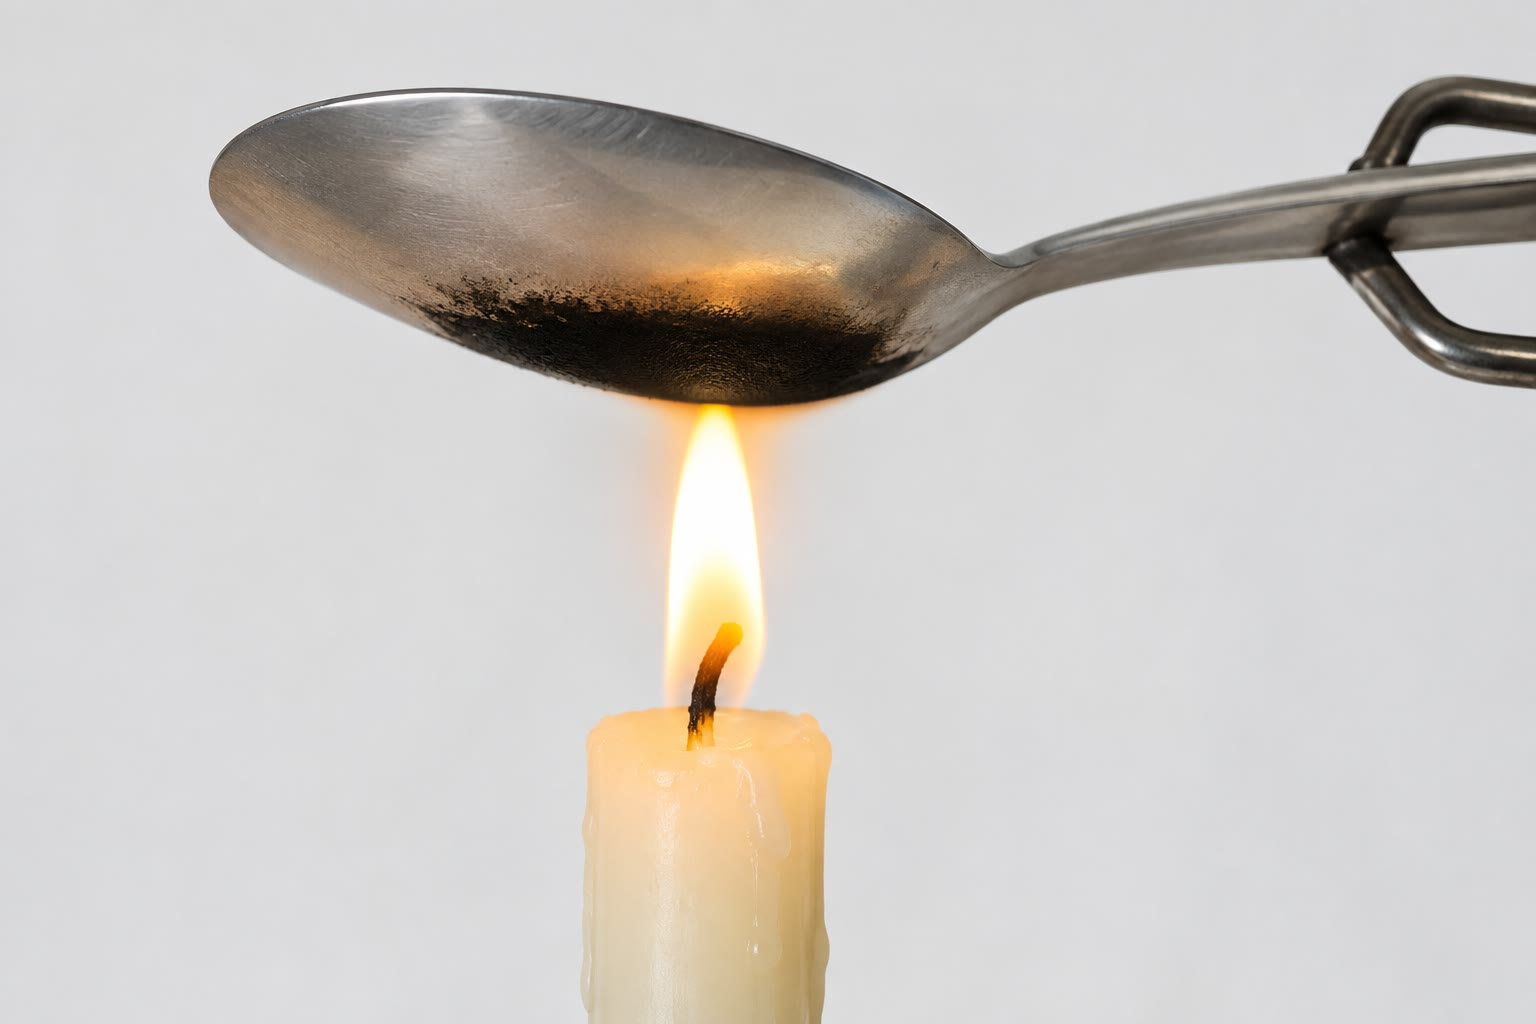
\includegraphics[width=0.45\linewidth]{images/book1/ai/g8-soot-spoon.jpg}

{\small 将一只冷勺子置于黄色烛焰中，被炭黑熏黑：
燃烧不完全。}
\end{omfigure}

\section{一氧化碳，无声的危险}

\begin{proposition}[一氧化碳为何致命]\label{prop:g8:combustion-and-fuels:co}
一氧化碳无色、无臭、无味。吸入后，它
会在血液中取代氧气（其机理在生物学教材中有解释），
引起头痛、嗜睡，在密闭房间中还会导致昏迷
乃至死亡。任何燃料在空气不足时燃烧都会产生它：燃气锅炉或
热水器维护不良或烟道堵塞，密闭帐篷中的炉子，
室内使用的烧烤炉或发电机。
\end{proposition}

\begin{safety}{\ghs[0.8cm]{GHS02}\ghs[0.8cm]{GHS04}\ghs[0.8cm]{GHS06}\ghs[0.8cm]{GHS08}}
% ledger: ghs:CO
一氧化碳：极易燃气体（GHS02），加压
储存（GHS04）；吸入有毒（GHS06）；长期或反复接触会损害器官
并可能危害未出生的胎儿（GHS08）。
\end{safety}

\begin{remark}[防止中毒]\label{rem:g8:combustion-and-fuels:prevent}
燃气用具应由专业人员定期维护，烟道
和进气口绝不能堵塞，烧烤炉和发电机只能在
室外使用，并且任何燃烧器附近都应安装一氧化碳报警器。
\end{remark}

\begin{omfigure}
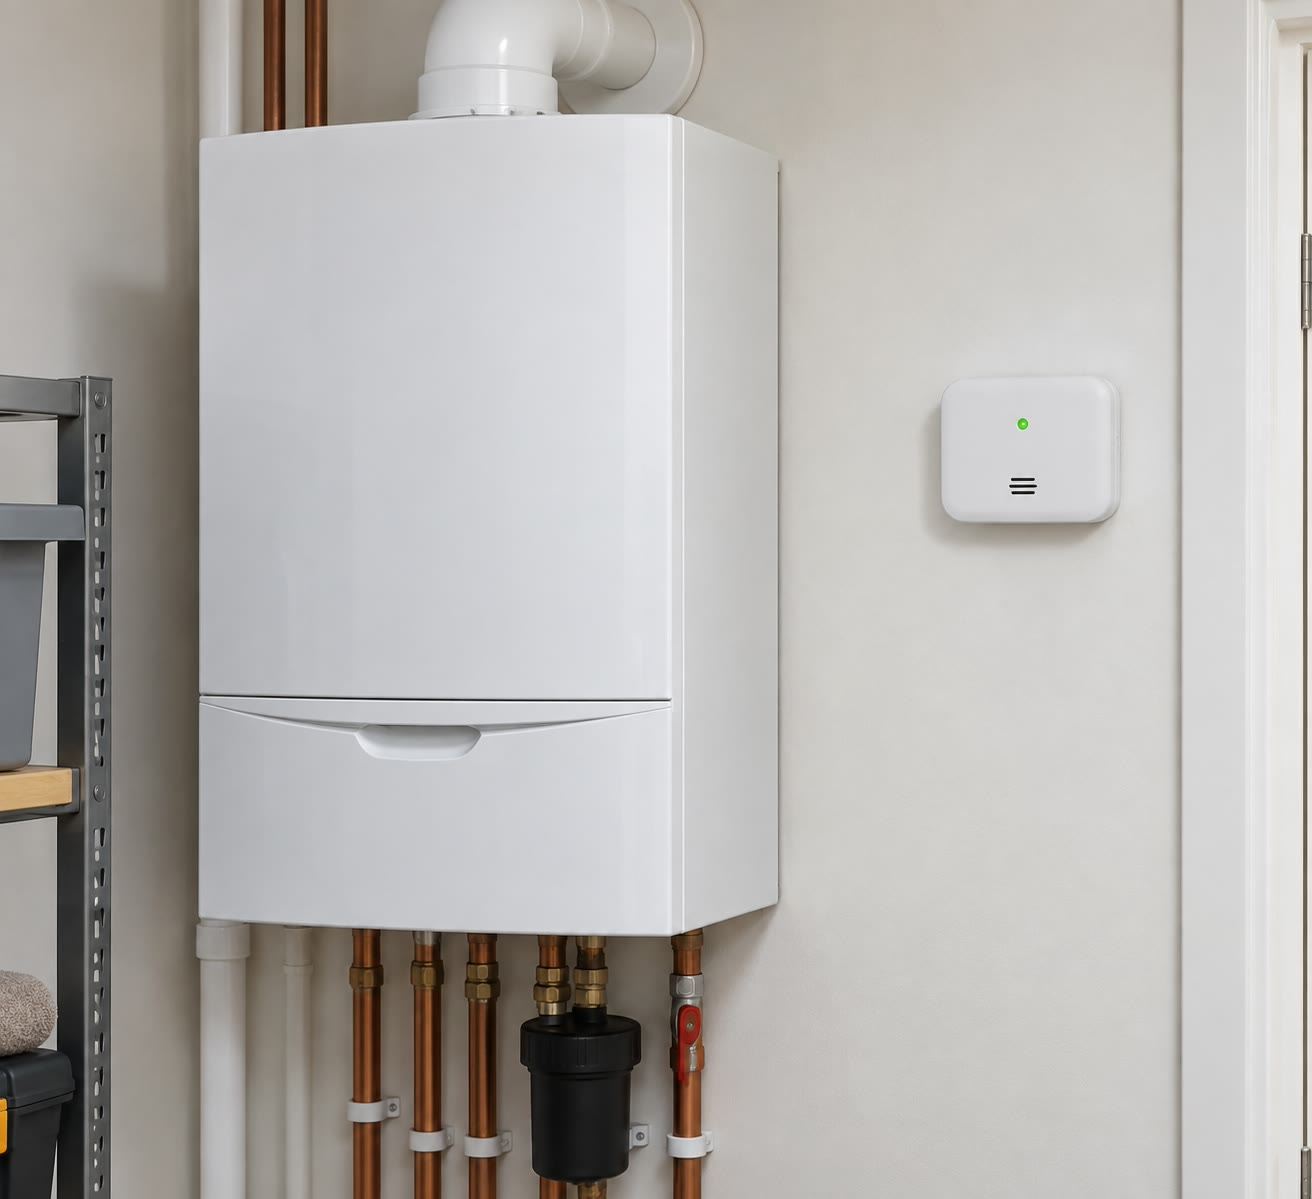
\includegraphics[width=0.45\linewidth]{images/book1/ai/g8-boiler-alarm.jpg}

{\small 一台燃气锅炉，旁边是一氧化碳报警器。}
\end{omfigure}

\section{二氧化碳与温室效应}

\begin{definition}[温室气体]\label{def:g8:combustion-and-fuels:greenhouse}
称\emph{温室气体}\index{温室气体}为空气中的一种气体，它允许阳光
穿过，却截留了地表向太空发射的部分热量，
从而使近地大气变暖。
水蒸气、二氧化碳和甲烷都是温室气体，氮气和氧气
则不是。
（其成因见物理教材。）
\end{definition}

\begin{proposition}[空气中的二氧化碳在不断增加]\label{prop:g8:combustion-and-fuels:rising}
% ledger: co2:mlo-1959, co2:mlo-2025 (rise 111.4 ppm, +35 %)
自 1959 年起，人们在太平洋中部一座山上的观测站上，
连续不间断地测量空气中的二氧化碳含量。
1959 年时，空气中二氧化碳含量为 316 ppm，
2025 年为 427 ppm：在人类一生的时间里，含量约上升了 \qty{35}{\percent}，
主要来自煤、石油和天然气的燃烧。多出的二氧化碳
加剧了温室效应，使气候变暖。
\end{proposition}

\begin{omfigure}
\begin{tikzpicture}
\begin{axis}[width=0.85\linewidth, height=6cm, xmin=1955, xmax=2030,
    ymin=300, ymax=440, xlabel={年份}, ylabel={二氧化碳（ppm）},
    axis lines*=left, ymajorgrids, grid style={gray!20},
    tick label style={font=\small, /pgf/number format/1000 sep={}},
    label style={font=\small}]
\addplot[omDef, thick, mark=*, mark size=0.8pt]
  table[x=year, y=ppm] {figdata/out/grade-8-co2-record.dat};
\node[anchor=west, font=\small] at (axis cs:1962,306) {1959 年为 316 ppm};
\node[anchor=east, font=\small] at (axis cs:2023,428) {2025 年为 427 ppm};
\end{axis}
\end{tikzpicture}

{\small 空气中二氧化碳的年平均含量，自 1959 年起测得
（NOAA 全球监测实验室数据；1974 年以前为
斯克里普斯海洋研究所数据）。}
\end{omfigure}

\section{化石燃料与可再生燃料}

\begin{definition}[化石燃料与可再生燃料]\label{def:g8:combustion-and-fuels:fossil}
\emph{化石燃料}\index{化石燃料}——煤、石油、天然气——
是在地下经数百万年，由古代植物和海洋生物的遗骸
形成的燃料。\emph{可再生燃料}\index{可再生燃料}是由当今生长的
植物或废弃物制成的燃料，包括木材、由粪便和食物废料制成的沼气，
以及由甜菜或甘蔗制成的乙醇。
\end{definition}

\begin{proposition}[碳从何而来]\label{prop:g8:combustion-and-fuels:cycle}
植物生长时从空气中吸收二氧化碳。燃烧可再生
燃料时，放出的二氧化碳是其植物几年前从空气中吸收的，
而燃烧化石燃料释放的碳，原本已被封存在地下数百万年，
会使空气中的二氧化碳增加。
\end{proposition}

\begin{omfigure}
\begin{tikzpicture}[font=\small,
    box/.style={draw=omDef, fill=omDef!6, rounded corners=2pt, align=center,
      minimum height=0.9cm, text width=2.6cm}]
  \node[box] (air) at (0,3) {二氧化碳 \\ 在空气中};
  \node[box] (plants) at (5.6,3) {植物生长 \\ （吸收 \ce{CO2}）};
  \node[box] (fuel) at (5.6,0.4) {木材、沼气、\\ 生物乙醇};
  \node[box, draw=black!50, fill=black!8] (fossil) at (0,0.4) {煤、石油、天然气：\\ 地下};
  \draw[->, thick, omProp] (air) -- (plants);
  \draw[->, thick, omProp] (plants) -- (fuel);
  \draw[->, thick, omProp] (fuel) -- (air);
  \node[text=black, font=\footnotesize, align=left, anchor=north west] at (1.5,1.45)
    {燃烧，\\ 数年后};
  \draw[->, thick, black!60] (fossil) -- node[midway, left, text=black, font=\footnotesize,
    align=right] {燃烧：\\ 碳储存 \\ 数百万年} (air);
\end{tikzpicture}

{\small 可再生燃料将其植物曾从空气中吸收的碳
重新释放回空气中；化石燃料则增加了原本储存在地下的碳。}
\end{omfigure}

\begin{omfigure}
\begin{minipage}[t]{0.48\linewidth}\centering
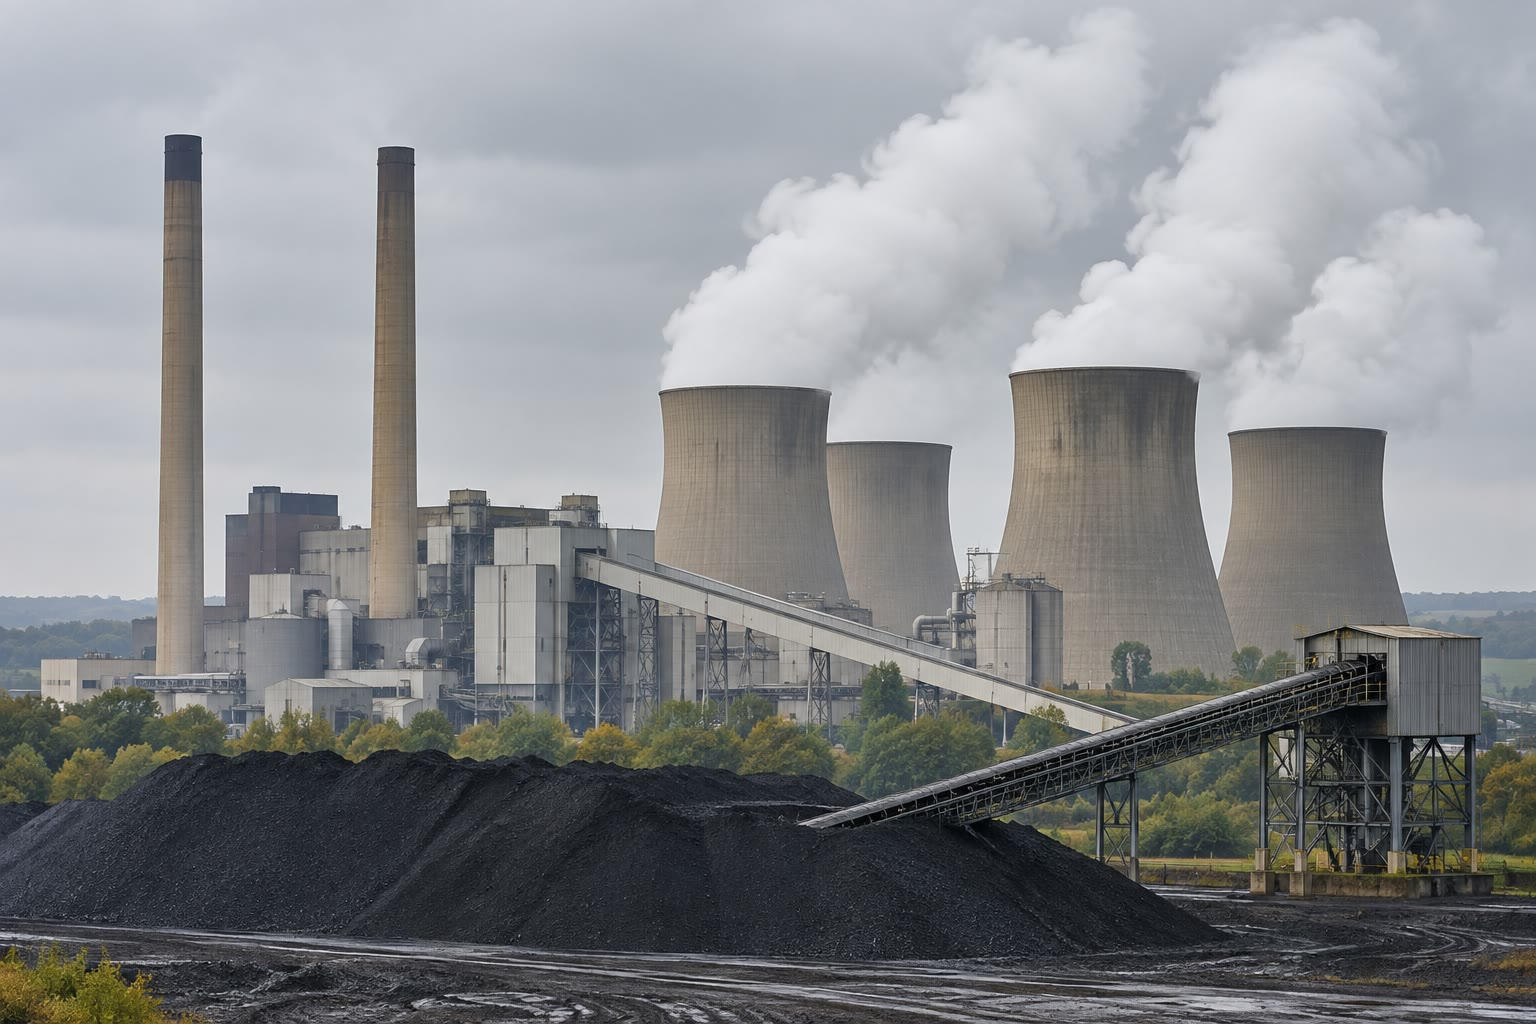
\includegraphics[width=\linewidth,height=4.6cm,keepaspectratio]{images/book1/ai/g8-coal-plant.jpg}

{\small 一座燃煤发电站。}
\end{minipage}\hfill
\begin{minipage}[t]{0.48\linewidth}\centering
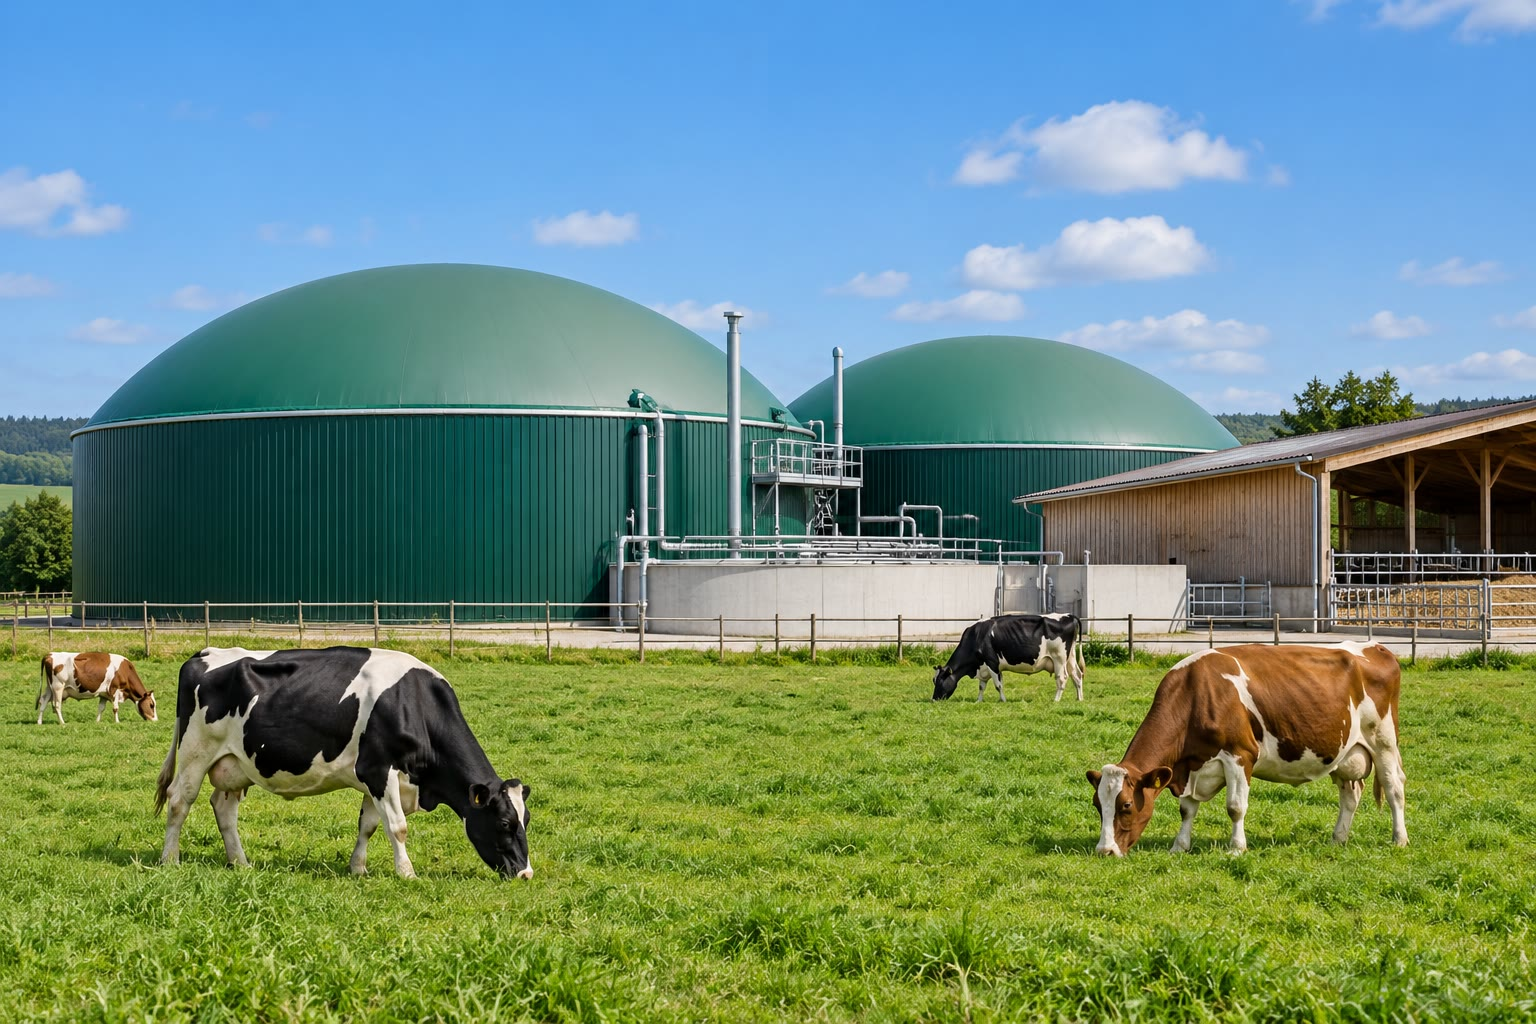
\includegraphics[width=\linewidth,height=4.6cm,keepaspectratio]{images/book1/ai/g8-biogas-farm.jpg}

{\small 一座农场沼气站：粪便变成了可再生燃料。}
\end{minipage}
\end{omfigure}

\section{练习}

\begin{exercise}[$\star$]\label{exo:g8:combustion-and-fuels:1}
写出碳完全燃烧的配平方程式。
\end{exercise}

\begin{exercise}[$\star$]\label{exo:g8:combustion-and-fuels:2}
完全燃烧与不完全燃烧有何区别？
\end{exercise}

\begin{exercise}[$\star$]\label{exo:g8:combustion-and-fuels:3}
为什么一氧化碳被称为“隐形杀手”？
\end{exercise}

\begin{exercise}[$\star$]\label{exo:g8:combustion-and-fuels:4}
判断下列燃料是化石燃料还是可再生燃料：煤、木材、天然气、沼气、汽油、
由甜菜制得的乙醇。
\end{exercise}

\begin{exercise}[$\star\star$]\label{exo:g8:combustion-and-fuels:5}
写出丙烷完全燃烧的配平方程式，
\ce{C3H8}.
\end{exercise}

\begin{exercise}[$\star\star$]\label{exo:g8:combustion-and-fuels:6}
乙醇 \ce{C2H6O} 在氧气中完全燃烧。配平下列方程式：
\ce{C2H6O + O2 -> CO2 + H2O}. % ce-unbalanced-ok (to balance)
\end{exercise}

\begin{exercise}[$\star\star$]\label{exo:g8:combustion-and-fuels:7}
将平底锅置于黄色火焰上方，锅底变黑。这种黑色
物质是什么？它说明了关于燃烧的什么情况？
\end{exercise}

\begin{exercise}[$\star\star$]\label{exo:g8:combustion-and-fuels:8}
读取二氧化碳曲线：在 1980 年和 2000 年，空气中
的二氧化碳含量大约是多少？这二十年间，二氧化碳含量
上升了多少 ppm？
\end{exercise}

\begin{exercise}[$\star\star$]\label{exo:g8:combustion-and-fuels:9}
为什么多年来，燃烧木材向空气中增加的二氧化碳
比燃烧煤少？虽然两者都会生成二氧化碳。
\end{exercise}

\begin{exercise}[$\star\star$]\label{exo:g8:combustion-and-fuels:10}
配平碳不完全燃烧生成一氧化碳的方程式：
\ce{C + O2 -> CO}. % ce-unbalanced-ok (to balance)
\end{exercise}

\begin{exercise}[$\star\star\star$]\label{exo:g8:combustion-and-fuels:11}
从 1959 年（316 ppm）到 2025 年（427 ppm），空气中的
二氧化碳含量增加了百分之几？结果四舍五入到整数。
\end{exercise}

\begin{exercise}[$\star\star\star$]\label{exo:g8:combustion-and-fuels:12}
在窗户紧闭的小房间里使用一台燃气取暖器。试用
本章的两个方程式说明，随着时间推移，燃烧如何由完全燃烧
转变为不完全燃烧，以及这为何危险。
\end{exercise}

\section{周末问题：帐篷中的炉子}

\begin{problem}[{周末问题——野营炉、它所燃烧的气体、
它生成的物质，以及它为什么绝不能放入帐篷内}]
\label{pb:g8:combustion-and-fuels:1}
% ledger: ghs:propane
野营炉燃烧的丙烷 \ce{C3H8} 取自一只气罐，气罐中装有
\qty{450}{g} 丙烷。在露天空气中，火焰呈蓝色。
由配平方程式算得以下质量比：\qty{44}{g} 丙烷
完全燃烧生成 \qty{132}{g} 二氧化碳。

\medskip
\noindent\textbf{第一部分——方程式。}
\begin{enumerate}
  \item 写出丙烷完全燃烧的
        方程式。
  \item 数一数方程式两边每种原子的数目，检验上一小题的结果。
  \item 配平下列不完全燃烧反应：
        \ce{C3H8 + O2 -> CO + H2O}. % ce-unbalanced-ok (to balance)
  \item 两者中，每个丙烷分子需要更多氧气的是哪一个？
\end{enumerate}

\medskip
\noindent\textbf{第二部分——在帐篷里。}
\begin{enumerate}[resume]
  \item 在封闭帐篷内点燃的炉子不久就会以黄色火焰燃烧。
        请解释其原因。
  \item 此时生成的是哪种有害气体？写出它的两条性质，
        这些性质使人难以察觉。
  \item 丙烷气罐上标有两个象形图，请写出它们的名称，
        并说明各自的含义。
  \item 写出两条安全使用野营炉的规则。
\end{enumerate}

\medskip
\noindent\textbf{第三部分——一个气罐中的二氧化碳。}
\begin{enumerate}[resume]
  \item 生成的二氧化碳质量是所燃烧丙烷质量的
        多少倍？
  \item 多出来的克数从何而来？
  \item 丙烷是化石燃料还是可再生燃料？燃烧丙烷是否会
        使空气中的二氧化碳增加？
  \item 计算整个
        \qty{450}{g} 气罐完全燃烧时释放的二氧化碳质量。
\end{enumerate}
\end{problem}
